%%%%%%%%%%%%%%%%%%%%%%%%%%%%%%%%%%%%%%%%%%%%%%%%%%%%%%%%%%%%%%%%%%%%%%%%%%%%%%%

\documentclass[12pt,twocolumn,tighten]{aastex62}
%\documentclass[12pt,twocolumn,tighten,trackchanges]{aastex62}
\usepackage{amsmath,amstext,amssymb}
\usepackage[T1]{fontenc}
\usepackage{apjfonts}
\usepackage[figure,figure*]{hypcap}
\usepackage{graphics,graphicx}
\usepackage{hyperref}
\usepackage{natbib}
\usepackage[caption=false]{subfig} % for subfloat
\usepackage{enumitem} % for specific spacing of enumerate
\usepackage{epigraph}

\renewcommand*{\sectionautorefname}{Section} %for \autoref
\renewcommand*{\subsectionautorefname}{Section} %for \autoref

\newcommand{\ptfo}{PTFO$\,$8-8695}
\newcommand{\ptfob}{PTFO$\,$8-8695b}

%% Reintroduced the \received and \accepted commands from AASTeX v5.2.
%% Add "Submitted to " argument.
\received{\today}
\revised{---}
\accepted{---}
\submitjournal{AAS journals.}
\shorttitle{Two Stars, Two Signals, No Planet}

\begin{document}

\defcitealias{bouma_wasp4b_2019}{B19}

% \title{Double, Double, Spin plus Nubble: Two Stars and Two Signals in
% PTFO 8-8695}
\title{PTFO 8-8695: Two Stars, Two Signals, No Planet}


\correspondingauthor{L.\,G.\,Bouma}
\email{luke@astro.princeton.edu}

%
% key authors:
%
\author[0000-0002-0514-5538]{L.\,G.\,Bouma}
\affiliation{Department of Astrophysical Sciences, Princeton
University, 4 Ivy Lane, Princeton, NJ 08540, USA}
%
\author[0000-0002-4265-047X]{J.\,N.\,Winn}
\affiliation{Department of Astrophysical Sciences, Princeton
University, 4 Ivy Lane, Princeton, NJ 08540, USA}
%
% 
%-------------------------------------
% TESS Mission Architects:
% These authors should be listed in this order
% see https://spacebook.mit.edu/pages/viewpage.action?pageId=24543276
%-------------------------------------
%
%CONFIRMED
\author{G. R. Ricker} % grr@space.mit.edu
\affiliation{Department of Physics and Kavli Institute for
Astrophysics and Space Research, Massachusetts Institute of
Technology, Cambridge, MA 02139, USA}
%
%CONFIRMED
\author[0000-0001-6763-6562]{R. Vanderspek} % roland@space.mit.edu
\affiliation{Department of Physics and Kavli Institute for
Astrophysics and Space Research, Massachusetts Institute of
Technology, Cambridge, MA 02139, USA}
%
%CONFIRMED
\author[0000-0001-9911-7388]{D. W.~Latham} % dlatham@cfa.harvard.edu
\affiliation{Center for Astrophysics \textbar \ Harvard \&
Smithsonian, 60 Garden St, Cambridge, MA 02138, USA}
%
%CONFIRMED
\author[0000-0002-6892-6948]{S.~Seager} % seager@mit.edu
\affiliation{Department of Physics and Kavli Institute for
Astrophysics and Space Research, Massachusetts Institute of
Technology, Cambridge, MA 02139, USA}
\affiliation{Department of Earth, Atmospheric and Planetary Sciences,
Massachusetts Institute of Technology, Cambridge, MA 02139, USA}
\affiliation{Department of Aeronautics and Astronautics, MIT, 77
Massachusetts Avenue, Cambridge, MA 02139, USA}
%
%CONFIRMED
\author[0000-0002-4715-9460]{J. M.~Jenkins} % jon.jenkins@nasa.gov
\affiliation{NASA Ames Research Center, Moffett Field, CA 94035, USA}
%
%-------------------------------------
% 3 representatives of each of SPOC, POC, TSO, for a total of 9. 
%These 9 authors should be listed in alphabetical order
%-------------------------------------
% 3 TSO COAUTHORS
%     Karen Collins karenacollins@outlook.com
%     Sam Quinn squinn@cfa.harvard.edu
%     Dana Louie danalouie@astro.umd.edu
% 3 SPOC COAUTHORS
%     Mark E. Rose mark.rose@nasa.gov
%     Jeffrey C. Smith  jeffrey.c.smith-1@nasa.gov
%     Bill Wohler  bill.wohler@nasa.gov
% 3 POC COAUTHORS: 
%     John Doty (jpd@noqsi.com)
%     Joel Villaseñor (jsvilla@space.mit.edu)
%     Tom Barclay (barclay.astro@gmail.com)

%CONFIRMED
\author[0000-0001-7139-2724]{T. Barclay} % barclay.astro@gmail.com
\affiliation{NASA Goddard Space Flight Center, 8800 Greenbelt Road,
Greenbelt, MD 20771, USA}
\affiliation{University of Maryland, Baltimore County, 1000 Hilltop
Circle, Baltimore, MD 21250, USA}

%CONFIRMED
\author[0000-0001-6588-9574]{K. A. Collins} % karenacollins@outlook.com
\affiliation{Center for Astrophysics \textbar \ Harvard \&
Smithsonian, 60 Garden St, Cambridge, MA 02138, USA}

%CONFIRMED
\author{J. P. Doty} % jpd@noqsi.com
\affiliation{Noqsi Aerospace Ltd., 15 Blanchard Avenue, Billerica, MA,
01821, USA}

%CONFIRMED
\author[0000-0002-2457-272X]{D.~R.~Louie} % danalouie@astro.umd.edu
\affiliation{Department of Astronomy, University of Maryland, College
Park, MD 20742, USA}

%CONFIRMED
\author[0000-0002-8964-8377]{S. N. Quinn} % squinn@cfa.harvard.edu
\affiliation{Center for Astrophysics \textbar \ Harvard \&
Smithsonian, 60 Garden St, Cambridge, MA 02138, USA}

%CONFIRMED
\author[0000-0003-4724-745X]{M. E. Rose} %  mark.rose@nasa.gov
\affiliation{NASA Ames Research Center, Moffett Field, CA 94035, USA}

%CONFIRMED
\author[0000-0002-6148-7903]{J. C. Smith} % jeffrey.c.smith-1@nasa.gov
\affiliation{NASA Ames Research Center, Moffett Field, CA 94035, USA}
\affiliation{SETI Institute, Mountain View, CA 94043, USA}

%CONFIRMED
\author{J. Villase\~nor} % jsvilla@space.mit.edu
\affiliation{Department of Physics and Kavli Institute for
Astrophysics and Space Research, Massachusetts Institute of
Technology, Cambridge, MA 02139, USA}

%CONFIRMED
\author[0000-0002-5402-9613]{B. Wohler} % bill.wohler@nasa.gov
\affiliation{NASA Ames Research Center, Moffett Field, CA 94035, USA}
\affiliation{SETI Institute, Mountain View, CA 94043, USA}


\begin{abstract}
  PTFO$\,$8-8695 (CVSO\,30) is a star in the 7--10 million year old
  Orion-OB1a cluster that shows brightness dips that resemble
  planetary transits.  While strong evidence against the planet
  hypothesis has already been provided, the possibility remains
  debated in the literature.  To obtain further clues, we inspected
  data from the NASA {\it Transiting Exoplanet Survey Satellite}
  (TESS) and the ESA Gaia mission.  The Gaia data show that
  PTFO$\,$8-8695 is a photometric binary with respect to members of
  its kinematic group, and independently suggest that it is an
  astrometric binary.  The TESS light curve shows two different
  photometric periods. The variability is dominated by a sinusoidal
  signal with a period of 11.98$\,$hr, presumably caused by stellar
  rotation.  Also present is a 10.76$\,$hr signal consisting of a
  not-quite sinusoid interrupted by hour-long dips, the type of signal
  previously intepreted as planetary transits.  The phase of the dips
  is nearly 180$^\circ$ away from the phase of the originally reported
  dips. As noted previously, this makes them difficult to explain as
  planetary transits.  Instead, we believe that PTFO$\,$8-8695 is a
  pair of young and rapidly rotating M dwarfs, one of which shows the
  same ``transient-dipper'' behavior that been seen in at least 5
  other cases.  The origin of these transient dips is still unknown
  but likely involves circumstellar material.
\end{abstract}

\keywords{
	Exoplanet evolution (491),
  Pre-main sequence stars (1290),
	Stellar ages (1581),
	Stellar rotation (1629),
	Variable stars (1761),
  Low mass stars (2050)
}

%%%%%%%%%%%%%%%%%%%%%%%%%%%%%%%%%%%%%%%%%%%%%%%%%%%%%%%%%%%%%%%%%%%%%%%%%%%%%%%


\section{Introduction}

We wish \ptfob\ were a planet. It would be quite exceptional. It would
be the youngest known hot Jupiter \citep{van_eyken_ptf_2012}, orbiting
a T Tauri star in the Orion-OB1a cluster.  It would have the shortest
orbital period of any hot Jupiter.  With such a short
period, it would probably be filling its Roche lobe, and actively
losing mass to its host star.  Not only that, but the rapidly-rotating
host star is probably oblate enough to torque the planet's orbit into
and out of the transiting configuration on a time scale of years
\citep{barnes_measurement_2013,ciardi_followup_2015,kamiaka_revisiting_2015}. 

Another first would be the direct detection of H$\alpha$ emission from
the planet itself \citep{johnskrull_h_2016}.  In addition to the
chromospheric H$\alpha$ emisson, it seems that there is an additional
H$\alpha$ emission with radial velocity variations in phase with the
planetary orbit.  The average velocity width of the excess H$\alpha$
emission is 87$\,$km$\,$s$^{-1}$, and its equivalent width is 70-80\%
that of the stellar chromosphere \citep{johnskrull_h_2016}.  The
proposed explanation is that the emission is from hot material flowing
away from the planet \citep{johnskrull_h_2016}.

However, the observed signals have some peculiarities that make the
planet seem even more unusual, to the point that they cast into doubt
the premise that \ptfob\ is real.  First, the transit-like brightness
dips are about three times deeper in optical bandpasses ({\it e.g.,}
$g$-band) than in the near-infrared ({\it e.g.}, $z$-band)
\citep{onitsuka_multicolor_2017,tanimoto_evidence_2020}.  An ordinary
atmosphere expected for a Jovian planet would not lead to such a
strong color-dependence of the transits.  Second, the planet does not
seem to emit as much infrared radiation as would be expected for such
a hot Jovian planet \citep{yu_tests_2015}.  Third, despite measurement
attempts by multiple investigators, \ptfob\ does not seem to show the
Rossiter effect at the amplitude expected given the rapid stellar
rotation and large planet size
\citep{yu_tests_2015,ciardi_followup_2015}.  Fourth, the phase of the
dips within the overall period of photometric variability has changed
drastically over the years since their initial discovery.  To counter
these objections, it has been proposed that the planet may be much
smaller than Jupiter and that the dips are produced by dust clouds
emitted from the planet \citep{tanimoto_evidence_2020}. 

A separate issue is that the brightness dips change shape over many
orbital cycles. This was initially explained by
\cite{barnes_measurement_2013} as the natural effects of gravity
darkening.  However, \cite{howarth_reappraisal_2016} argued that the
necessary amplitude of gravity darkening is too large to be realistic,
given the spectroscopically-determined rotation velocity.
Additionally, as the gravity-darkened star precessed about its
rotation axis, it would show photometric variability that has not been
observed.

While the planetary interpretation clearly faces challenges, there is
no completely satisfactory alternate explanation.  High-latitude
accretion hotspots might produce the observed H$\alpha$ variability,
but require fine-tuning to produce dips of the appropriate duration.
Furthermore, \ptfo\ does not have an infrared (IR) excess associated
with the presence of dust at the inner edge of a primordial disk
\citep[{\it e.g.},][Figure~18]{yu_tests_2015}.  Low-latitude
starspots, hot or cold, struggle to produce photometric features as
short as some of the observed dips.

A relevant fact is that between 0.1\% and 1\% of rapidly rotating
low-mass stars in $\mathcal{O}$(10)$\,$Myr old associations show
short-duration dips as part of their overall periodic variability
\citep{rebull_usco_2018}.  The dips can persist over months, but their
depths often vary, and sometimes change immediately after stellar
flares.  The explanation proposed by \citet{stauffer_orbiting_2017}
and \citet{david_transient_2017} to explain this novel class of
variable stars is that a circumstellar cloud of gas is orbiting near
the co-rotation radius.  To this point, though, it has not been clear
if this explanation applies to \ptfo, because the determination of the
stellar rotation period has been somewhat ambiguous
\citep{van_eyken_ptf_2012,koen_multicolour_2015,raetz_yeti_2016}.

We begin in Section~\ref{sec:observations} by describing newly
available observations from TESS \citep{ricker_transiting_2015} and
Gaia \citep{gaia_collaboration_gaia_2018}.  The TESS light curve shows
two different periodic signals, which we analyze in
Section~\ref{sec:tess}.  The Gaia data, analyzed in
Section~\ref{sec:gaia}, show that \ptfo\ is a photometric binary and
suggest it is also an astrometric binary.  We discuss the pieces of
the puzzle in Section~\ref{sec:discussion}, and summarize the
situation in Section~\ref{sec:conclusions}.  We comment on the study
by \citet{koen_2020} in postscript.



\section{The Data}
\label{sec:observations}

\begin{figure*}[t!]
	\begin{center}
		\leavevmode
		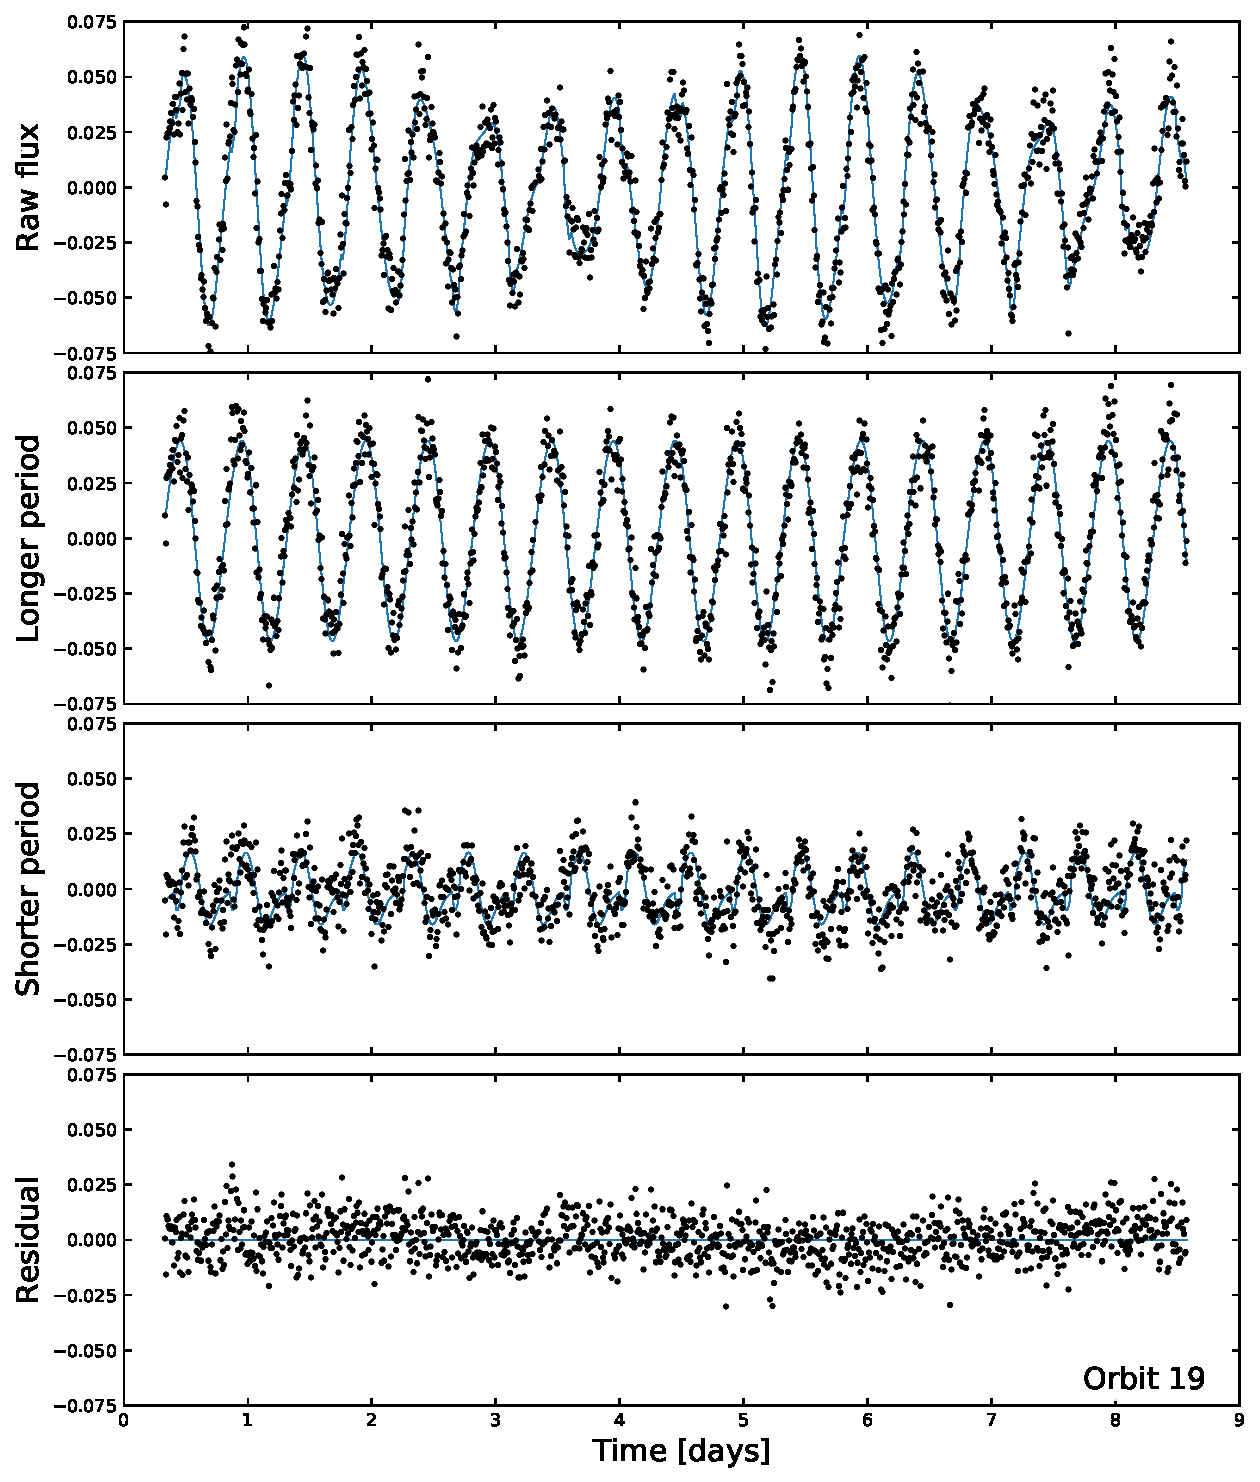
\includegraphics[width=1\textwidth]{f1.pdf}
	\end{center}
	\vspace{-0.7cm}
	\caption{
    {\bf TESS light curve of \ptfo\ (Sector 6, Orbit 19).} {\it Top}:
    The original (\texttt{PDCSAP} mean-subtracted) relative flux.
    The beat period of 4.48 days is visible by eye.  The blue curve is
    a model including 2 harmonics at the longer period $P_{\rm \ell}$,
    plus 3 harmonics and a transit at the shorter period $P_{\rm s}$.
    {\it Upper middle}: Longer-period signal, equal to the original signal
    minus the shorter-period signal.  {\it Lower middle}:
    Shorter-period signal, equal to the original signal minus the
    longer-period signal.  {\it Bottom}: residual relative flux.  The
    data are binned from 2 to 10 minute cadence as a convenience for
    plotting and fitting.
		\label{fig:splitsignal}
	}
\end{figure*}

\begin{figure*}[hbtp]
	\begin{center}
		\leavevmode
		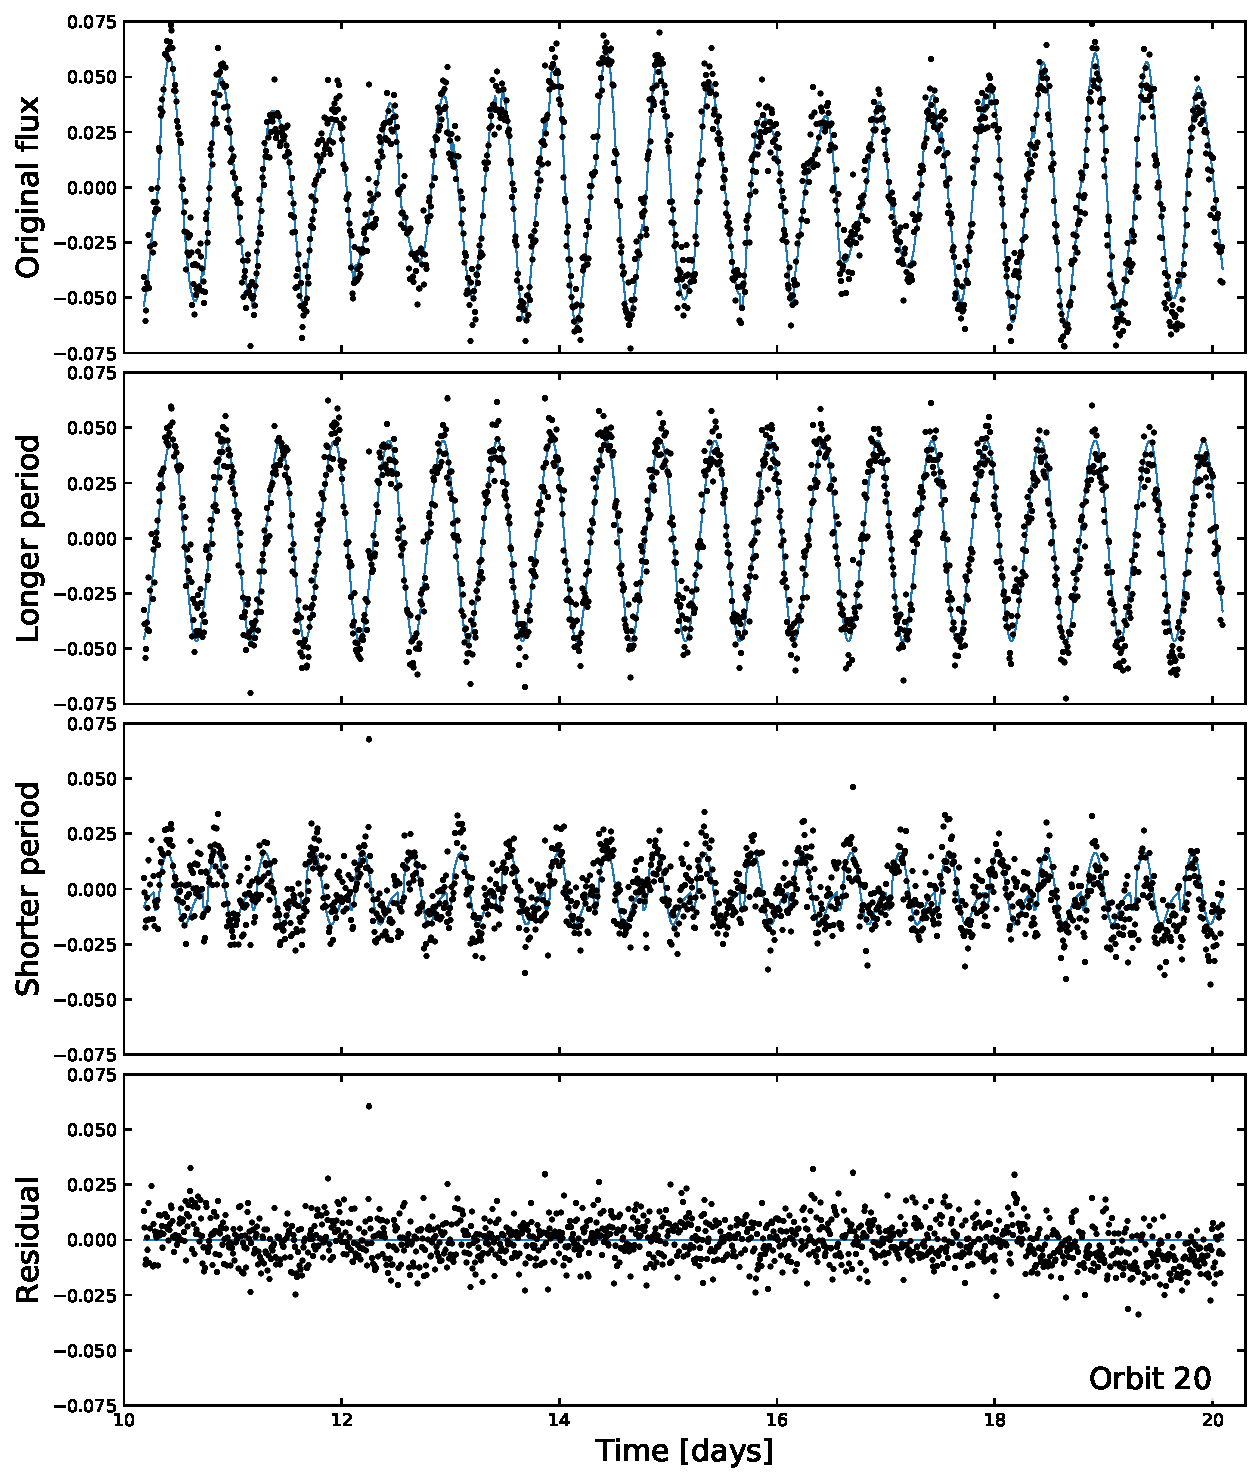
\includegraphics[width=1\textwidth]{f2.pdf}
	\end{center}
	\vspace{-0.7cm}
  \caption{ {\bf TESS light curve of \ptfo\ (Sector 6, Orbit 20).} Same
  format as Figure~\ref{fig:splitsignal}.
  \label{fig:splitsignalii}
	}
\end{figure*}

\subsection{TESS Observations}

\ptfo\ (also known as CVSO\,30; \citealt{briceno_cida_2005}) was
observed by TESS with Camera 1, CCD 1, from December 15, 2018 until
January 6, 2019, during the sixth sector of science operations
\citep{ricker_transiting_2015}.  The star was designated
TIC\,264461976 in the TESS Input Catalog
\citep{stassun_TIC_2018,stassun_TIC8_2019}.  The pixel data for an
$11\times11$ array surrounding \ptfo\ were averaged into 2-minute
stacks by the onboard computer.  Each 2048$\times$2048 image from the
CCD was also averaged into 30-minute stacks, and saved as a ``full
frame image'' (FFI).

The 2-minute stacks for \ptfo\ were reduced to light curves by the
Science Processing Operations Center (SPOC) at NASA
Ames~\citep{jenkins_tess_2016}.  We mainly used the Presearch Data
Conditioning (PDC) light curve.  The PDC light curve aperture used
pixels chosen to maximize the SNR of the total flux of the target
\citep{bryson_2020_target_aperture}.  Non-astrophysical variability
was removed by fitting out trends common to many stars
\citep{smith_kepler_2012,stumpe_multiscale_2014}.
% \citep{smith_kepler_PDC_2017}
% \citep{smith_kepler_apertures_2017}

As an independent check on the 2-minute SPOC light curve, we examined
the light curve based upon 30-minute image stacks which was produced as
part of the Cluster Difference Imaging Photometric Survey (CDIPS;
\citealt{bouma_cluster_2019}).  Our CDIPS light curve of choice used a
circular aperture with radius 1 pixel.

To clean the data, we removed all points with non-zero quality flags,
which indicate known problems \citep[{\it
e.g.},][]{tess_data_product_description_2018}.  We also masked out the
data from the first and last 6 hours of each orbit, since there are
often systematic red noise in the photometry during those times.  Both
the CDIPS and PDC light curves showed a clear discontinuous jump in the
last few days of orbit 20, which seemed likely to be an instrumental
systematic effect.  We correspondingly masked out the data with
timestamps ranging from BJD\,2458488.3 until the end of the orbit.
The PDC light curve initially had 15{,}678 points.  The quality-flag
cut removed 854 points; masking the orbit edges removed an additional
716 points; and removing the data from the final few days of orbit 20
removed an additional 1079 points.  After cleaning, 83\% of the
initial flux measurements remained.

We normalized the light curve by dividing out the median flux, and then
opted to subtract 1{.}0 to set the median value to zero, which
simplified subsequent interpretation.  Many of these and subsequent
processing steps were performed using
\texttt{astrobase}~\citep{bhatti_astrobase_2018}. 


\subsection{Gaia Observations}

\subsubsection{Astrometric measurements}

Between July 25, 2014 and May 23, 2016, Gaia measured about 300
billion centroid positions of 1{.}6 billion stars
\citep{gaia_collaboration_gaia_2016,lindegren_gaiasoln_2018,gaia_collaboration_gaia_2018}.
In the Gaia second data release (DR2), these CCD observations were
used to determine positions, proper motions, and parallaxes of the
brighest 1{.}3 billion stars, including \ptfo\
\citep{lindegren_gaiasoln_2018}.  For \ptfo, there were 121 ``good''
observations, {\it i.e.}, observations that were not strongly
down-weighted in the astrometric solution.  \ptfo\ was assigned the
Gaia DR2 identifier 3222255959210123904.  Its photometric brightness
was measured using selected bands ($G$, $Rp$, and $Bp$) of the Gaia
Radial Velocity Spectrometer
\citep{cropper_gaia_2018,evans_gaia_2018}.  We accessed the pipeline
parameters for \ptfo\ using the Gaia
archive\footnote{\url{gea.esac.esa.int/archive/}}.

The majority of Gaia's derived parameters for \ptfo\ agreed with
expectations from former studies
\citep{briceno_cida_2005,van_eyken_ptf_2012}.  The main novelty is
that Gaia DR2 reported a 10.3$\sigma$ ``astrometric excess'',
indicating that the residuals to the best-fitting astrometric model
were larger than expected based on the statistical uncertainties.  We
comment on the significance and interpretation of this excess in
Section~\ref{sec:gaia}.


\subsubsection{Hierarchical Cluster Membership}
\label{subsec:hierarchical}

Gaia also provided astrometric parameters for tens of thousands of
young stars in the Orion complex.  Stellar populations in giant
molecular cloud complexes are not monolithic; substructured groups are
the norm \citep{briceno_lowmassOB_2007}.  The Orion molecular cloud
complex in particular has numerous subgroups, with ages ranging from
0.5 to 15$\,$Myr. For an incomplete sampling, see for instance
\citet{briceno_cida_2005,jeffries_kinematic_2006,briceno_25_2007,kounkel_apogee2_2018}
and \citet{briceno_cidaII_2019}.

\ptfo\ was initially identified as a member of the Orion$\,$OB1a
sub-association and designated CVSO\,30 by \citet{briceno_cida_2005}
through combined photometry and spectroscopy.  Later work by
\citet{briceno_25_2007} clarified that \ptfo\ was in a kinematically
distinct subgroup of Orion~OB1a, named the ``25$\,$Ori'' group after
its brightest member. They reported that the 25$\,$Ori group has an
isochrone age of 7--10$\,$Myr, and a smaller fraction of stars with
disks than younger nearby sub-associations
\citep{hernandez_spitzer_ob1_2007}.

With the Gaia astrometry, it has become clear that 25$\,$Ori itself
has distinct subgroups
\citep{kounkel_apogee2_2018,briceno_cidaII_2019}.  In describing the
cluster membership of \ptfo, we follow the notation and results of
\citet{kounkel_apogee2_2018}.  These authors combined astrometric data
from Gaia DR2 with near-infrared spectra from APOGEE-2
\citep{gunn_sdss_2006,majewski_apache_2017,blanton_sloan_2017,zasowski_target_2017,cottle_apogee2_2018}.
They performed a hierarchical clustering on the six-dimensional
position and velocity information to identify subgroups within the
Orion complex.  From smallest to largest, \ptfo\ was identified as a
member of the following hierarchical subgroups:
\begin{equation}
  {\rm 25\,Ori\text{-}1}
  \subset {\rm 25\,Ori}
  \subset {\rm Orion\ OB1a}
  \subset {\rm Orion\ D},
\end{equation}
where `$\subset$' means ``is a proper subset of''.  25$\,$Ori-1 is the
largest subgroup of 25$\,$Ori, with 149 identified members.  Based on
the color-magnitude diagram (CMD), the mean age was found to be
6.9$\,$Myr, while the HR diagram led to an estimated age of 8.5$\,$Myr
\citep[see][Section 2.3]{kounkel_apogee2_2018}.
\citet{kounkel_apogee2_2018} identified seven other smaller groups in
the Orion complex near the Be star 25$\,$Ori. These groups received
higher numbers, {\it e.g.}, 25$\,$Ori-2 (${\rm Age}_{\rm CMD}
=15.1\,$Myr; ${\rm Age}_{\rm CMD} =12.9\,$Myr; see also
\citealt{briceno_cidaII_2019}).

These details concerning the group membership for one object are
cumbersome to those accustomed to the simple distinction between
``young cluster members'' and ``old field stars''.  Although all
members of the Orion complex are indeed young relative to the field,
these details are essential for assessing the photometric evidence for
the binarity of \ptfo, because of the degeneracy between stellar
luminosity and age for pre-main-sequence stars.  Having a clean sample
of reference stars that are tightly associated with \ptfo\ --- both
spatially and kinematically --- minimizes contamination not only from
field stars, but also from older and younger members of the Orion
complex.


\section{TESS Analysis}
\label{sec:tess}

\begin{figure*}[t]
	\begin{center}
		\leavevmode
		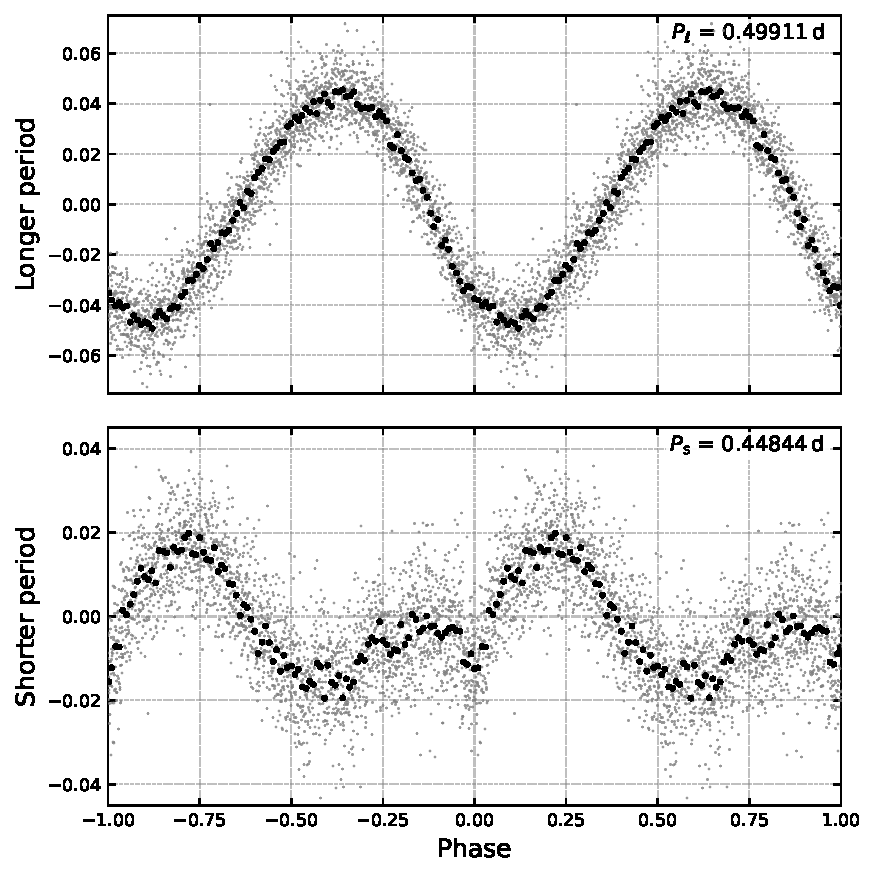
\includegraphics[width=1\textwidth]{f3.pdf}
	\end{center}
	\vspace{-0.7cm}
	\caption{ {\bf Phase-folded longer and shorter-period signals.}
    {\it Top}: Relative flux at the longer period, as in
    Figure~\ref{fig:splitsignal}.  {\it Bottom}: Relative flux at the
    shorter period. The reference phase is set to the dip.  Gray
    points are the 10 minute cadence \texttt{PDCSAP} flux.  Black
    points are binned to 100 points per period.
    The model (blue line)
    includes 2 harmonics at the longer period,
    plus 3 harmonics and a transit at the shorter period.
		\label{fig:phasefold}
	}
\end{figure*}

\subsection{Inspection}

Our initial inspection of the TESS light curve, in both its 2-minute
PDCSAP and 30-minute FFI forms, showed a strong sinusoidal beat signal
(Figures~\ref{fig:splitsignal} and~\ref{fig:splitsignalii}, top
panel). As a precursor to more detailed analysis, we calculated
generalized Lomb-Scargle periodograms using \texttt{astrobase}
\citep{lomb_1976,scargle_studies_1982,vanderplas_periodograms_2015,bhatti_astrobase_2018}.
The two tallest peaks occur at 0.448\,d (10.76$\,$hr) and 0.499\,d
(11.98$\,$hr).  We will refer to these two periods as the ``shorter
period'' $P_{\rm s}$ and the ``longer period'' $P_{\rm \ell}$.  The
peak at $P_{\rm \ell}$ is the taller of the two peaks.  Lower-power
harmonics of both signals are also present.

% 0.14 = A1+A2
% 0.06 = A1-A2
% 2A1 = 0.20
% -> A1 = 0.1
% 2A2 = 0.08
% -> A2 = 0.04

The peak-to-peak light curve amplitude at maximum, when the two signals
interfere constructively, is about 14\%.  During the times of
destructive interference, the peak-to-peak amplitude is about 6\%.
Assuming the signals are mainly sinusoidal, simple algebra tells us
that the peak-to-peak amplitudes should be about 10\% for the
longer-period signal, and 4\% for the shorter-period signal.  To view
the phase-folded light curves of the longer-period signal, we
subtracted the best-fitting sinusoid at the shorter period; the
resulting light curve appears smooth and nearly sinusoidal.  But after
subtracting the best-fitting sinusoid at the longer period, visual
inspection of the phase-folded light curve of the shorter-period
signal revealed substructure resembling the ``dips'' seen in previous
observations. In particular, there was a $\approx$1\% dip lasting
about an hour.  These initial impressions turned out to be consistent
with the results of our more complicated analysis, described below.


\subsection{Light Curve Model}

We fitted a model to the light curve consisting of a linear combination
of Fourier modes with periods $P_{\rm s}$ and $P_{\rm \ell}$, as well
as a number of harmonics chosen as described below. To try accounting
for the dips, we also added an analytic transit model with period
$P_{\rm s}$.  Symbolically, the total flux $f$ is given as
\begin{equation}
  f = f_{\rm s} + f_{\rm \ell}
  = f_{\rm transit,s} + f_{\rm Fourier,s} + f_{\rm Fourier,\ell},
\end{equation}
where $f_{\rm s}$ is the flux at the shorter period, and $f_{\rm
\ell}$ is the flux at the longer period.  Writing out the Fourier
terms explicitly,
\begin{align}
  f = &f_{\rm transit,s} + \sum_{n=1}^{N_{\rm s}} A_n \sin(n\omega_{\rm s}t)
  + \sum_{n=1}^{N_{\rm s}} B_n \cos(n\omega_{\rm s}t)\\
  &+ \sum_{m=1}^{N_{\rm \ell}} A_m \sin(m[\omega_{\rm \ell}t+\phi_{\rm \ell}])
  + \sum_{m=1}^{N_{\rm \ell}} B_m \cos(m[\omega_{\rm \ell}t+\phi_{\rm \ell}]), \nonumber
\end{align}
where $N_{\rm s}$ and $N_{\rm \ell}$ are the total number of modes at
the shorter and longer periods, respectively, $A_i$ and $B_i$ are the
amplitudes of each mode (which can be positive or negative), and
$\omega_\ell$ and $\omega_{\rm s}$ are the angular frequencies of the
longer-period and shorter-period signals. By not including a phase
parameter in the shorter-period model, we have implicitly defined the
zero point of the phase scale. The relative phase of the longer-period
model is specified by the phase parameter $\phi_\ell$.  Since we did
not know in advance how many harmonics would be appropriate to include
in the model, we considered a number of different choices for $N_{\rm
s}$ and $N_{\rm \ell}$, and used the Bayesian information criterion to
select the final model (Table~1).

As an example, one possible model consists of a transit, $N_{\rm s}=2$
sines and cosines at the shorter period, plus $N_{\rm \ell}=1$ sine
and cosine at the longer period.  In this case, the free parameters
would be as follows.  The transit model parameters are the impact
parameter, the planet-to-star radius ratio, two quadratic limb
darkening parameters, the planet's orbital period (set equal to
$P_{\rm s}$) the time of a particular transit, and the mean flux.  We
also independently sampled the stellar radius and mass, implicitly
defining the stellar density.  Additionally, there would be $2N_{\rm
s}=4$ additional Fourier amplitudes at the shorter period, plus
$2N_{\rm \ell}=2$ Fourier amplitudes at the longer period, as well as
$P_\ell$ itself and the relative phase $\phi_\ell$.  The total number
of parameters would be 17.

We implemented and fitted the models using \texttt{PyMC3}, which is
built on \texttt{theano}
\citep{salvatier_2016_PyMC3,exoplanet:theano}.  For the Fourier terms,
we used the default math operators.  For the exoplanet transit, we
used the model and derivatives implemented in the \texttt{exoplanet}
code \citep{exoplanet:exoplanet}.  Our priors are listed in Table~2.
To speed up the fitting process, we averaged the 2-minute light curve
to 10-minute samples.  We correspondingly scaled the uncertainties in
the flux measurements by a factor of $\sqrt{5}$.  Before sampling, we
initialized each model with the parameters of the maximum {\it a
posteriori} (MAP) model.  We then assumed a Gaussian likelihood, and
sampled using \texttt{PyMC3}'s gradient-based No-U-Turn Sampler
\citep{hoffman_no-u-turn_2014}, and used $\hat{R}$ as our convergence
diagnostic \citep{gelman_inference_1992}.  We tested our ability to
successfully recover injected parameters using synthetic data before
fitting the \ptfo\ light curves.


\subsection{Fitting Results}

We considered nine models, with the number of modes per frequency
$N_{\rm s}$ and $N_{\rm \ell}$ ranging from one to three.  To select
our preferred model, we used the Bayesian information criterion
(Table~1).  The model with the lowest BIC had three modes at the
shorter 10.76$\,$hr period, and two modes at the longer 11.98$\,$hr
period.
The other models had BIC values that implied significantly less
support \citep{burnham_multimodel_2016}.
All nine models have
reduced $\chi^2$ values ranging between 1.21 and 1.68, which suggests
a plausible though imperfect agreement between the data and the model
to within the formal uncertainties.  Table~2 gives the best-fitting
parameters for the preferred model, which has the lowest BIC value.

To explore where each model succeeded and failed, we split the
original signal into its respective components
(Figures~\ref{fig:splitsignal} and~\ref{fig:splitsignalii}).  We also
examined the phase-folded signals (Figure~\ref{fig:phasefold}).  

In every model, the 11.98$\,$hr variability is a simple sinusoid
with peak-to-peak amplitude $\approx$10\%.  The 10.76$\,$hr
variability is always more complex.  The overall impression is of a
distorted sinusoidal function, with a peak-to-peak amplitude of about
4\%.  The asymmetric sinusoid rises to a maximum near phase 0.25, and
reaches minimum brightness between phases $-0.5$ and $-0.25$.  Between
phases $-0.5$ and $0.0$ there appears to be complex shorter-timescale
variability, ending with a ``dip'' of depth $\approx$1.2\%, lasting
$\approx$0.75 hours.  The fact that our preferred model has three
rather than two ``short period'' harmonics is linked to the degree of
curvature required between phases $-0.5$ and $-0.05$: the analogous
$(N_{\rm \ell},N_{\rm s})=(2,2)$ model prefers a longer transit duration,
but does not fit the out-of-transit curvature as well, particularly
immediately before ingress.

The periodogram of the final residual shows a barely significant and
poorly-resolved peak at $\approx$8 days, consistent with the visual
impression of some slower trends in the bottom rows of
Figures~\ref{fig:splitsignal} and~\ref{fig:splitsignalii}.

\section{Tests for Binarity}
\label{sec:gaia}

\subsection{Visual Binarity}
\label{subsec:blend}

\begin{figure}[t]
	\begin{center}
		\leavevmode
		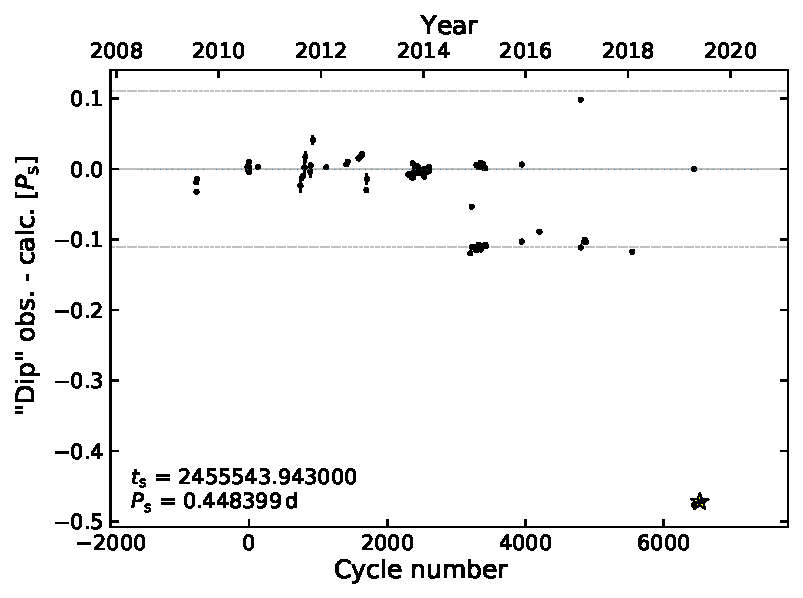
\includegraphics[width=0.45\textwidth]{f4.pdf}
	\end{center}
	\vspace{-0.7cm}
	\caption{ {\bf Scene used for blend analysis.}
    {\it Top:} Mean TESS image of \ptfo\ over Sector~6, with a
    logarithmic grayscale. The yellow star is the position of \ptfo.
    Orange crosses are neighboring stars with $T<17$. The \texttt{X}
    and \texttt{/} hatches show the apertures used to measure the
    background and target star flux, respectively.  {\it Bottom:}
    Digitized Sky Survey $R$-band image of the same field, with a
    linear grayscale. The circles show the apertures of radii 1, 1.5,
    and 2.25 pixels used in our blend analysis. To the northwest of
    \ptfo\ and between the blue and orange circles is ``Star A'', the
    only star bright and close enough to be contributing to the signal
    attributed to \ptfo. However, the pixel-level TESS data showed
    that Star A is not the source of the observed variability (see
    Section~\ref{subsec:blend}).
		\label{fig:scene}
	}
\end{figure}

The TESS pixels are $\approx21$'' per side. Before making any
interpretations, we needed to consider whether light from neighboring
stars could have contributed to the photometric signal we are
attributing to \ptfo. The scene is shown in Figure~\ref{fig:scene}.
In the upper panels, the pixels used to measure the background level
in the SPOC light curve are indicated with `\texttt{X}' hatching, and
the pixels used in the final light curve aperture are shown with
`\texttt{/}' hatching.

The target star, \ptfo\ (TIC 264461976), has a $T$-band magnitude of
14.0, and its position is shown with a star.  The other (unlabeled)
star inside the target aperture, TIC 264461979, has $T=16.8$ and so
cannot contribute more than about 10\% to the total signal.  The only
neighbor that is sufficiently close and bright that its light might
contaminate the target star is TIC 264461980, with $T=14.8$, which we
dub ``Star A''.  Star A is 23.6'' northwest of the target, and based
on the magnitude difference could contribute flux variations as large
as 48\% the flux of our target star, \ptfo.  

The variability of \ptfo\ with a period consistent with $P_{\rm s}$
had already been observed based on images with arcsecond resolution.
Thus, our main concern regarding blending was whether the
longer-period signal with period $P_{\rm \ell}$ originated from \ptfo,
or from Star A. We took two approaches to investigate the source of
the long-period signal.

First, we examined the CDIPS FFI light curves of the target, which are
available on MAST \citep{bouma_cluster_2019}. Three light curves are
available, based on photometric apertures with a radius of 1, 1.5, or
2.5 pixels. The maximal peak-to-peak beat amplitude was the same to
within a percent, regardless of the size of the photometric aperture
that was used to create the light curve.  If Star A were the source of
the long-period variability, we would expect the peak variability
amplitude to be smallest in the 1 pixel aperture, based on the
separation of the sources (Figure~\ref{fig:scene}, bottom).  From this
test alone, it seems unlikely that Star A is the source of the
long-period signal.

Second, we examined the 2-minute light curve of each individual pixel
in the scene, using the interactive tools implemented in
\texttt{lightkurve} \citep{lightkurve_2018}.  If Star A were the
source of the long-period variability, we would expect the pixels
nearest to Star A to show a sinusoidal signal with amplitude exceeding
$10\%$.  The data do not show this pattern.  The pixel directly below
Star A does not clearly show any sinusoidal variability; the
peak-to-peak variability in that pixel is $\lesssim 8\%$.  In
contrast, the south-easternmost pixel within the \ptfo\ aperture (the
pixel furthest from Star A that was used in the optimal aperture)
shows the longer-period sinusoidal variability signal with an
amplitude of 14\%.  We conclude that within the resolution of the Gaia
DR2 source catalog, the $P_{\rm s}$ and $P_{\rm \ell}$ signals
originate from \ptfo.  Based on the work of
\citet{ziegler_measuring_2018}, we can surmise that stellar companions
with separations wider than $\approx$1'' (349~AU) and within $\Delta G
\approx 3$ magnitudes of \ptfo\ would have likely been detected
through this approach. 

Stronger constraints on possible
stellar companions were obtained by
\citet{van_eyken_ptf_2012} through high-resolution imaging with the NIRC2
camera on Keck II.  They reported 3-$\sigma$ $H$-band magnitude
difference limits of 4.3, 6.4, and 8.9 at angular separations of 0.25,
0.5, and 1.0 arcseconds (87, 175, and 349~AU).  They also detected a
point source, not present in Gaia DR2, 7.0 magnitudes fainter than the
target, and 1.8$''$ to the north-east.  Due to the brightness
difference, this point source\footnote{This point source was claimed
to be a potential planetary-mass object \citep{schmidt_direct_2016}.
Subsequent analysis of its colors showed that it is a background star
\citep{lee_evidence_2018}.} cannot be the source of our signals.


\subsection{Photometric Binarity}

\begin{figure*}[t]
	\begin{center}
		\leavevmode
		\subfloat{
			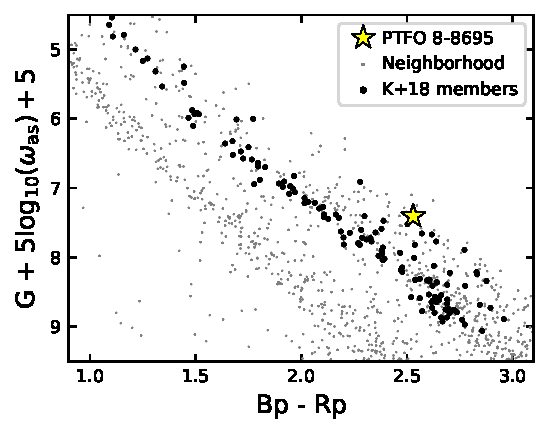
\includegraphics[width=0.7\textwidth]{f5a.pdf}
		}
		
		\vspace{-0.7cm}
		\subfloat{
			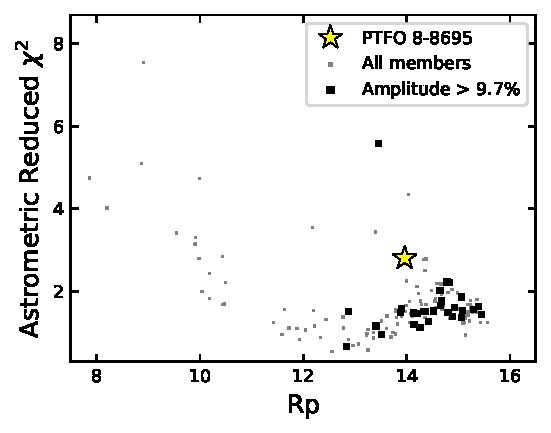
\includegraphics[width=0.7\textwidth]{f5b.pdf}
		}
	\end{center}
	\vspace{-0.7cm}
	\caption{ {\bf Evidence for binarity in \ptfo}.
    {\it Top:} Hertzsprung-Russell diagram of \ptfo\ and late-type
    members of 25$\,$Ori-1. Members of the 25$\,$Ori-1 group (black
    circles) were identified by \citet{kounkel_apogee2_2018}.  The
    gray circles are stars in the ``neighborhood'', i.e., non-member
    stars within 5 standard deviations of the mean 25$\,$Ori-1 right
    ascension, declination, and parallax.  It contains members of the
    Orion complex with its full spread of ages, in addition to field
    interlopers.  $G$ denotes Gaia broadband magnitudes, $Bp$ Gaia
    blue, $Rp$ Gaia red, and $\omega_{\rm as}$ the parallax in
    arcseconds.  The $x$-axis limits are set to show only K and M
    dwarfs, to accentuate \ptfo's separation from the single-star
    sequence.  {\it Bottom:} Astrometric goodness-of-fit versus $Rp$
    magnitude for 25$\,$Ori-1 members.  The single-source astrometric
    model for \ptfo\ provides a poor fit, which could be due to
    stellar variability or binarity.  Cluster members that are at
    least as variable as \ptfo\ show lower astrometric excesses (black
    squares), suggesting binarity as the root cause.
		\label{fig:gaia}
	}
\end{figure*}


We also used the Gaia data to see if the observed luminosity of \ptfo\ 
is too bright to be a single star, i.e., if it is a ``photometric
binary.'' To assemble a set of stars coeval with \ptfo, we used the
25$\,$Ori-1 members identified by \citet{kounkel_apogee2_2018}, and
discussed in Section~\ref{subsec:hierarchical}.

To define a set of non-member stars that nonetheless are subject to
similar selection criteria, we defined the reference ``neighborhood''
as the group of at most $10^4$ randomly selected non-member stars
within 5 standard deviations of the mean 25$\,$Ori-1 right ascension,
declination, and parallax.  We queried Gaia DR2 for these stars using
\texttt{astroquery} \citep{astroquery_2018}.  This yielded 1{,}819
neighbors.  While some of these stars may indeed be members of the
Orion complex, or even of 25$\,$Ori-1, enforcing this cut on positions
and parallaxes ensures that we are comparing stars with similar
amounts of interstellar reddening.

We examined the resulting five-dimensional distribution of right
ascension, declination, proper motion in both directions, and
parallax.  The first point we noted was that 25$\,$Ori-1 is a clearly
defined over-density in each dimension: the cluster was confirmed to
exist, and to be distinct from the neighborhood. \ptfo\ was also
within the cluster in each of these projected dimensions.

Figure~\ref{fig:gaia} shows the HR diagram we constructed from the
data.  The diagram shows that \ptfo\ is $\approx$0.75 magnitudes
brighter than the average 25$\,$Ori-1 star of the same color.  In
other words, it is about twice as bright as expected for a single star
in the cluster.  It also seems to be part of a ``photometric binary''
track that runs parallel to the main track.

The implication is that either {\it (i)} \ptfo\ is notably younger
than the kinematically identical 25$\,$Ori-1 members, or {\it (ii)}
\ptfo\ is a binary with two components of nearly equal brightness.
Since there is no other reason to suspect an age difference, and
because the source showed two separate photometric signals with
similar but distinct periods, the binary interpretation seems more
probable.

\subsection{Astrometric Binarity}

A separate possible line of evidence for binarity is the Gaia DR2
astrometry.  As noted in Section~\ref{sec:observations}, the Gaia DR2
astrometric solution for \ptfo\ shows a 10.3$\sigma$ ``astrometric
excess'', a parameter that quantifies the degree to which a
single-star model fails to fit the astrometric measurements.
Specifically, the single-source astrometric model yielded
$\chi^2=325.2$.  There are 121 astrometric measurements, and 5 free
parameters, and therefore 116 degrees of freedom. The reduced $\chi^2$
is 2.80.  The majority of stars with comparable brightness in Gaia do
not show such poor goodness-of-fit \citep[see][Appendix
A]{lindegren_gaiasoln_2018}.

Potential explanations for the poor astrometric fit include
photometric variability and unresolved stellar binarity \citep[{\it
e.g.},][]{rizzuto_ZEIT8_2018,belokurov_unresolved_2020}.  If
photometric variability were the cause, we would expect comparably
faint stars in the same kinematic group of Orion to show similar
astrometric excesses, as the majority of young stars are highly
variable.

% NB: CDIPS-I only made 131 light curves for 25Ori-1, because I wasn't
% aware of the Kounkel+18 member list at the time.
Using the same 149 members in the 25$\,$Ori-1 subgroup, we calculated
the astrometric reduced $\chi^2$ for each member.  We then queried the
CDIPS light curve database at MAST \citep{bouma_cluster_2019} to find
the subset of members that were at least as variable as \ptfo.  We
measured the variability amplitude by taking the difference between
the $95^{\rm th}$ and $5^{\rm th}$ percentiles of the flux
measurements.  This yielded 30 stars of equal or greater variability.
The lower panel of Figure~\ref{fig:gaia} shows the reduced $\chi^2$ as
a function of stellar brightness.  \ptfo\ is in the upper 90$^{\rm
th}$ percentile of stars showing astrometric excesses within the
25$\,$Ori-1 group.  Relative to other M-dwarf group members with
comparable brightnesses and variability characteristics, \ptfo\ still
stands out by virtue of its failure to conform to a single-star
astrometric model. This supports the interpretation that \ptfo\ is a
binary star.

Performing the same analysis using the renormalized unit weight error
(RUWE\footnote{ See the Gaia DPAC technical note
GAIA-C3-TN-LU-LL-124-01,
\url{http://www.rssd.esa.int/doc_fetch.php?id=3757412}, accessed
2020-04-27. }) rather than the reduced $\chi^2$ yielded similar
results.  \ptfo\ has a RUWE of 1{.}22, which corresponds to the
93$^{\rm rd}$ percentile of 25$\,$Ori-1 members.  Two of thirty stars
with variability amplitudes greater than 9.7\% showed higher RUWE.
One was CVSO~35, which has a TESS light curve that varies by 2
magnitudes, and shows a strong IR excess and a 10$\mu$m silicate emission
feature \citep{mauco_herschel_2018}.  The other is GAIA DR2
3222210363837122048.

We will have to wait for the full release of the nominal Gaia mission
to determine definitively whether the astrometric excess is caused by
stellar binarity or photometric variability.  Nonetheless the fact
that comparably variable stars do not show comparably large
astrometric excesses suggests that stellar binarity is indeed the root
cause.

\subsection{Radial Velocity Binarity}

Long-baseline radial velocity (RV) measurements could also reveal
the presence of multiple stars in this system.
Unfortunately,
the available RV data for \ptfo\ is rather sparse, presumably due to the
stellar faintness and equatorial velocity.
The RV datasets with the longest baselines we could find
in the literature were those reported by \citet{van_eyken_ptf_2012}.
These included 5 Keck/HIRES measurements acquired
over 10 days in April 2011, and 4 HET/HRS measurements acquired over
10 days in February 2011.  The root-mean-squared RV over each 10 day
span was $\approx$$2\,{\rm km}\,{\rm s}^{-1}$, consistent with the
measurement precision.  Although \citet{van_eyken_ptf_2012} tried a
CCF-based RV reduction technique, they eventually found that manually
selecting absorption lines and measuring line centroids was more
effective.  While \citet{yu_tests_2015} acquired 22 further Keck/HIRES
spectra over one night in December 2013, those points were not reduced
to velocities, and it is not clear whether the appropriate calibration
data exist.  Further Keck/HIRES measurements of \ptfo, if
appropriately calibrated, could potentially confirm or refute the
presence of binary companions.

\section{Discussion}
\label{sec:discussion}

\subsection{Longer-Period Signal}

The standard interpretation for 11.98$\,$hr nearly sinusoidal
modulations of a pre-main-sequence M dwarf is stellar rotation.  This
is the dominant signal in the system with 10\% amplitude, and there is
no evidence to suggest that this signal has any other origin.

In their report on the discovery of the unusual photometric
variability, \citet{van_eyken_ptf_2012} saw an alias of the
longer-period signal ({\it e.g.}, their Figure~7), and identified it
as a periodogram peak at $0.9985 \pm 0.0061\,$days. They ascribed it
to their observing cadence, because of its close correspondence to the
sidereal day.  Our pixel-level analysis showed that the signal is
specific to only pixels near \ptfo, and no other pixels.  We therefore
conclude that the signal is not an artifact of systematic errors.

We are not the first to reach the conclusion that the long period
sinusoidal modulation is astrophysical.  A study by
\citet{koen_multicolour_2015} identified the same modes and aliases as
\citet{van_eyken_ptf_2012}, but argued that the signal was
astrophysical (however they were still unsure of the exact period).
Using photometry from the YETI global telescope network,
\citet{raetz_yeti_2016} eventually came to the conclusion that the
$0.50\,{\rm d}$ signal was indeed from stellar rotation.  The TESS
data strongly support this conclusion.



\subsection{Shorter-Period Signal, Including the ``Dip''}

\begin{figure}[t]
	\begin{center}
		\leavevmode
		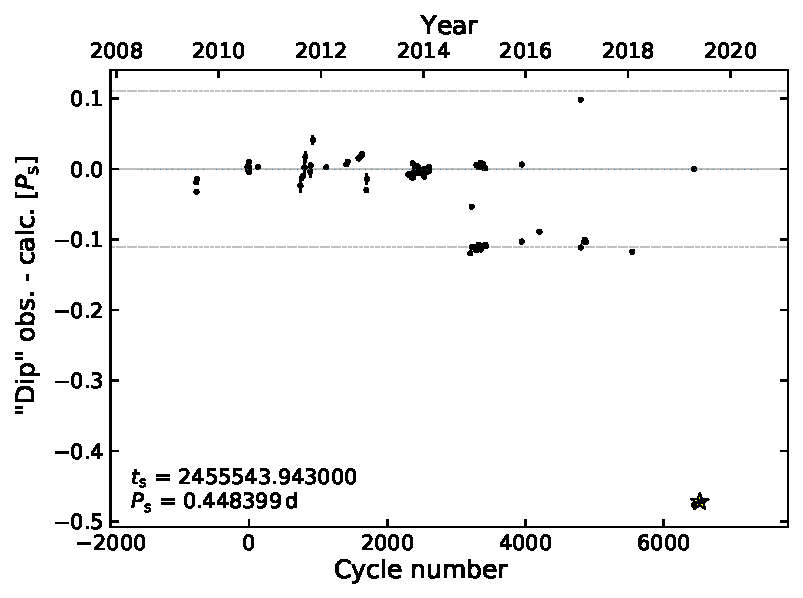
\includegraphics[width=0.5\textwidth]{f6.pdf}
	\end{center}
	\vspace{-0.7cm}
	\caption{
    {\bf Timing residuals for \ptfob\ based on a decade of
    monitoring.} Black points are times of dips, minus the indicated
    linear ephemeris.  The phase of the shorter-period signal is
    plotted on the $y$-axis. The star symbol represents the TESS
    ephemeris.  Dips were observed by \citet{van_eyken_ptf_2012},
    \citet{ciardi_followup_2015}, \citet{yu_tests_2015},
    \citet{raetz_yeti_2016}, \citet{onitsuka_multicolor_2017}, and
    \citet{tanimoto_evidence_2020}.  Certain dips ({\it e.g.}, the one
    at phase 0 in mid-2019) are consistent with noise, and were likely
    reported because dips were expected, rather than convincingly
    observed.  Horizontal dashed lines are drawn at $\pm (P_{\rm \ell}
    - P_{\rm s})/P_{\rm s}$, highlighting either a numerical
    coincidence or an observational bias.  The orbital phase observed
    by TESS (lower-right) is consistent with that of
    \citet{tanimoto_evidence_2020}.
		\label{fig:o_minus_c}
	}
\end{figure}

The TESS light curve shows a dip that lasts about 45 minutes, and seems
to recur every 10.76 hours
(Figures~\ref{fig:splitsignal},~\ref{fig:splitsignalii},~\ref{fig:phasefold}).
The dip duration is roughly the same as that observed by previous
investigators \citep{van_eyken_ptf_2012,yu_tests_2015}.  The 1.2\%
depth is similar to what has been observed in the near-infrared
\citep{onitsuka_multicolor_2017}.  However the dip depth seems likely
to have evolved over time between being not present at all, to a
maximum of $\approx$5\% \citep[{\it
e.g.},][]{koen_multicolour_2015,yu_tests_2015,tanimoto_evidence_2020}.

One particularly interesting feature of the dip is its epoch.  The
dips do not occur with strict periodicity \citep{yu_tests_2015}.  In
fact, \citet{tanimoto_evidence_2020} provided stark evidence for
different behavior altogether: over a time-span of years, the dip
``split'' into distinct groups at particular repeating phases.  See
for instance their Figures~2 through~4.  Fitting a decade of
observations, they provided the following linear ephemeris, which we
did not find any need to update.
\begin{align}
t_0\ {\rm BJD}_{\rm TDB} &= 2455543.943 \pm 0.002 \nonumber \\
P &= 0.4483993 \pm 0.0000006\,{\rm d}.
\label{eq:ephem}
\end{align}

Figure~\ref{fig:o_minus_c} shows the observed mid-transit times of
dips minus the times predicted from Equation~\ref{eq:ephem}.  The
phase of the dip we detected in the TESS data (yellow star) agrees
with the independent December 2018 measurements by
\citet{tanimoto_evidence_2020}: either the dip abruptly shifted phase
over the past decade or, more likely, there are multiple dips that
have come and gone at different phases.

Figure~\ref{fig:o_minus_c} shows two additional strange features: {\it
(i)}  multiple dips per cycle, and {\it (ii)} a set of dips
numerically coincident with phase $(P_{\rm \ell} - P_{\rm s}) / P_{\rm
s}$.  The observation of multiple dips per cycle in 2015 was seen
independently by both \citet{yu_tests_2015} and
\citet{tanimoto_evidence_2020}.  It therefore seems credible.
Inspecting the \citet{tanimoto_evidence_2020} light curves, the claim
of multiple dips per cycle in December 2018 at phase 0 and $-0{.}47$
seems less plausible---the phase $\text{-}0{.}47$ dips are strongly
detected, while the suggested phase 0 dip is not clearly present in
the data.

We are not sure what to make of the numerical coincidence.  The ratio
of long to short periods is roughly 10:9.  It is not clear that this
would obviously translate into an observational bias unless by some
fluke three season's worth of observations managed to only observe
every ninth dip.  This is of course not the case, and we therefore
leave this curiosity as observation {\it sans} interpretation.
% JNW: This seems like an important clue. I don't have the mental
% energy to ponder it now, but it deserves pondering.


\subsection{Short Period Out-of-Dip Modulation}

Visually, the out-of-dip modulation at the 10.76$\,$hr period
resembles a slightly asymmetric sinusoid (Figure~\ref{fig:phasefold}).
Non-zero contributions in both the first and second harmonics are
detected (Table~2).  The first sine and cosine harmonic both have
amplitudes of roughly $0.90\pm0.04\%$.  The second sine harmonic has
amplitude $0.16 \pm 0.04\%$, so is non-zero at a significance of
$\approx$4$\sigma$.  The second cosine harmonic has negative amplitude $0.55
\pm 0.03\%$.  In our sign convention, the fact that it is negative
means that this component peaks at phase 0.25 and 0.75.

\subsubsection{Ellipsoidal Variability?}
If there were a giant planet transiting \ptfo, it would tidally
distort the host star, and cause ellipsoidal photometric modulations
that also peak at quadrature \citep[see][]{shporer_astrophysics_2017}.
Interpreting the second cosine harmonic as planet-induced tidal
distortion, it would imply a minimum planet mass $M_{\rm p} \sin i$ of
$3.8\,M_{\rm Jup}$.  For this estimate, we assumed $R_\star = 1.39
R_\odot$, and $M_\star = 0.39 M_\odot$ \citep{van_eyken_ptf_2012}.
This ellipsoidal amplitude is larger than the typical modulations
induced by close-in giant planets because the host star is puffy, and
still on the pre-main-sequence.

The planetary interpretation however does not readily explain the
large first sine and cosine harmonics.  Interpreting the sine component as
Doppler beaming would imply a secondary mass greater than the primary
($0.86\,M_\odot$).  Interpreting the cosine component as reflected or
emitted light from the planet's surface is nonsensical because the
sign is wrong---the planet would need to be {\it absorbing} light.

\subsubsection{Similar Light Curves}
\label{subsec:dipstars}

\begin{figure*}[hbtp]
	\begin{center}
		\leavevmode
		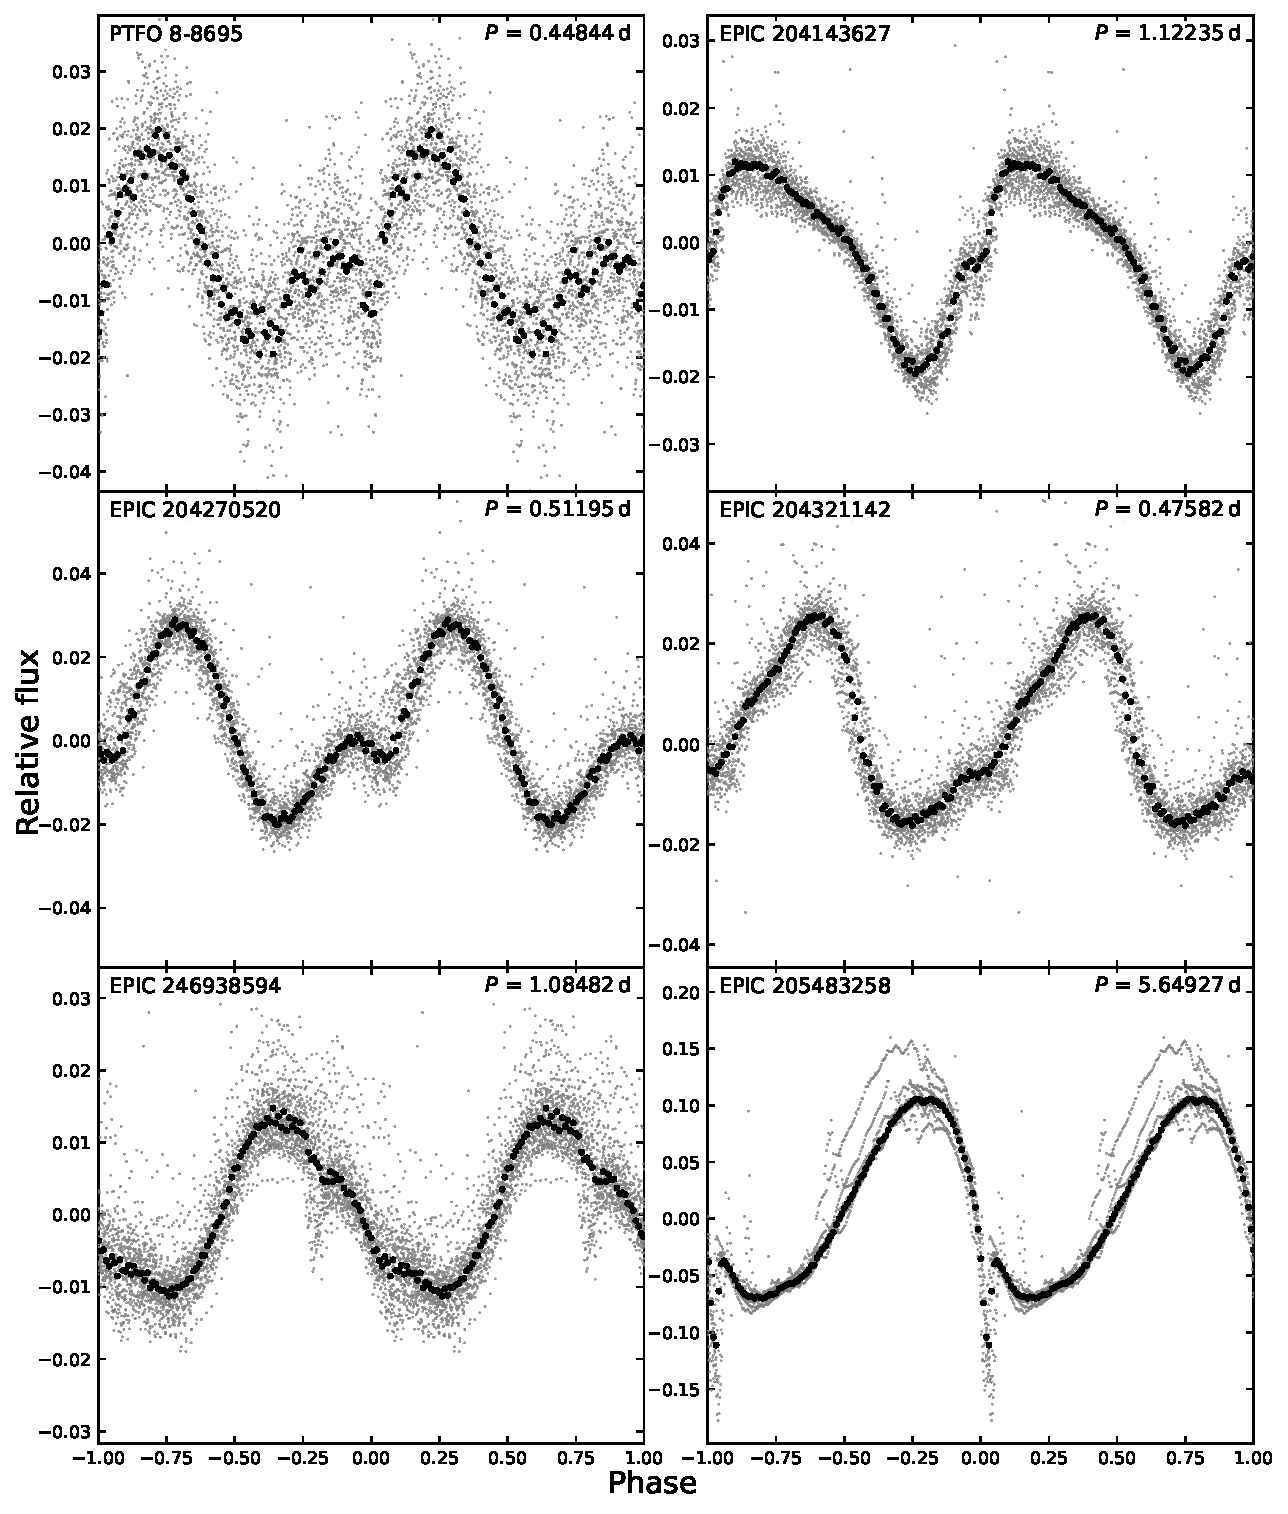
\includegraphics[width=1\textwidth]{f7.pdf}
	\end{center}
	\vspace{-0.7cm}
  \caption{ {\bf \ptfo\ and its brethren.}
    Five transient and persistent flux dip stars selected based on
    their visual similarity to the short-period signal in \ptfo\ are as
    shown.
    They include
    EPIC 204143627,
    EPIC 204270520,
    EPIC 204321142,
    EPIC 246938594,
    and
    EPIC 205483258 (RIK-210).
    RIK-210 has the longest period of any of these objects.  All the
    analogs displayed are either in Taurus or Upper~Sco, and meet the
    characteristics of Section~\ref{subsec:dipstars}.  We found these
    objects through studies by \citet{stauffer_orbiting_2017},
    \citet{david_transient_2017}, and \citet{rebull_usco_2018}.
		\label{fig:brethren}
	}
\end{figure*}

When physical explanations are not forthcoming, taxonomy is a useful
exercise.  By searching the literature, we have found about a dozen
light curves with similar morphologies to \ptfo, drawn from surveys of
low-mass weak-lined T Tauri stars in regions including $\rho$ Oph,
Upper~Sco, Taurus, and perhaps the Pleiades
\citep{rebull_rotation_2016,david_transient_2017,stauffer_orbiting_2017,stauffer_rotevol_2018,rebull_usco_2018,rebull_rotation_2020}.
These surveys were performed using K2 \citep{howell_k2_2014}.  We
downloaded some of these light curves from MAST, opting for the EVEREST
reductions \citep{luger_everest_2016,luger_update_2018}.  They are
plotted in Figure~\ref{fig:brethren}.

These light curves have been phenomenologically classified as
``persistent flux dips'' or ``transient flux dips'', based on whether
their depths and durations show variability over the 90-day K2
campaigns \citep{stauffer_orbiting_2017}.  In the terminology of
\citet{stauffer_orbiting_2017}, these objects are morphologically
distinct from ``scallop shell'' light curves, and are present in stars
at more advanced evolutionary disk stages than the ``dipper'' stars
\citep{ansdell_young_2016,cody_manyfaceted_2018}.  The persistent and
transient flux dip stars all show angular dips that are cannot be
explained as the effects of starspots.  These stars typically have the
following things in common:
\begin{enumerate}[topsep=0.5ex,itemsep=-0.5ex,partopsep=1ex,parsep=1.5ex]
  \item They are weak-lined T Tauri stars.
  \item The spectral type is M2 to M5 ({\it e.g.},
    \citealt{rebull_usco_2018},~Figure~20).
  \item The age is typically\footnote{
    At present, the oldest observed ``scallops'' are in the Pleaides
    \citep{rebull_rotation_2016}. One of these, EPIC 211013604, might
    meet the ``persistent dip'' classification.  If so, it is also the
    oldest known.
    } $\lesssim$ 100$\,$Myr.
  \item The light curves show shallow, angular dips, usually superposed
    on large-amplitude smooth variability. The latter is interpreted
    as stellar rotation.
  \item The rotation is rapid---usually between 0.5 and 2.0 days.
  \item There is rarely any detectable infrared excess in WISE data
  (never any W4 detection; only a few W3 detections).
  \item They sometimes show multiple dips per cycle.
  \item The dip depths, durations, and phases can vary over just a few
    cycles ({\it e.g.}, EPIC 204143627).
  \item The dip depths can change after flares.
  \item They are rare at a population level: $\lesssim 1\%$ of relevant stars
    \citep{rebull_usco_2018}.
\end{enumerate}
The 10.76$\,$hr signal in \ptfo\ meets all of these criteria.  This is
the first connection of \ptfo\ with this class of objects because the
TESS light curve was needed to resolve the different rotation signals.

There are two crucial additional points concerning the transient flux
dips.  First, the dip durations seem to scale linearly with the
photometric periods \citep[][Figure~26]{stauffer_orbiting_2017}.  In
the usual idealized limits, the transit duration $T$ of a point source
across the stellar disk scales as $T \propto R_\star
(P/M_\star)^{1/3}$ \citep{winn_exoplanet_2010}.  While the shortest
period $\approx$0.5-day transient flux dip stars have dip durations
consistent with point sources, at longer periods of 1 to 5 days the
dip durations become many hours, far too long to be caused by
planetary transits.

Second, between 40-50\% of the transient flux dip stars discovered in
$\rho$~Oph and Upper~Sco show two Lomb-Scargle periods, and so are
apparently binaries \citep[][Table~1]{stauffer_orbiting_2017}.  This
is higher than the main-sequence companion fraction of ${\rm
CF}_{0.1\text{-}0.5\,M_\odot}^{\rm MS} = 33 \pm 5\%$
\citep{henry_solar_2006,duchene_stellar_2013,winters_solar_2019}.
Low-mass pre-main-sequence stars however have been shown to companion
fractions up to twice as high in dispersed clusters such as Upper~Sco
and Taurus \citep{kraus_mapping_2008,kraus_mapping_2011}.  A detailed
high-resolution imaging survey would be necessary to determine whether
the transient flux dip stars truly have any distinct population-level
binarity properties relative to other young low-mass stars.


\subsection{Physical Interpretation}
\label{subsec:physical}

The evidence for binarity in \ptfo\ is as follows.  First, the star is
photometrically twice as bright as stars of the same color in its
kinematic group (Figure~\ref{fig:gaia}).  Second, it shows two
distinct photometric signals.  These points alone suggest binarity
\citep{stauffer_rotevol_2018}.  For the case of \ptfo, there is a
third line of evidence: the Gaia DR2 entry for \ptfo\ reports a poor
fit of the single-star model to the astrometric data.  While this
could be caused by stellar variability, other cluster members that are
just as variable do not typically show the same level of excess
astrometric motion.  Therefore the astrometric excess is a suggestive
third line of evidence for binarity in \ptfo. To us, the evidence
leads to the conclusion that \ptfo\ is a nearly equal-mass binary
consisting of two rapidly rotating stars.

Based on the lack of an infrared excess seen by \citet{yu_tests_2015},
the primordial gas disks seem to be have been depleted\footnote{A
potential confounding factor is completeness. Is Spitzer sensitive to
infrared excesses at the distance of Orion? The series of studies by
\cite{hernandez_spitzer_2006,hernandez_spitzer_ob1_2007,hernandez_spitzer_sig_2007,hernandez_spitzer_2009}
show that it is.} around both stars in \ptfo. The stars are therefore
no longer magnetically locked to their disks.  This is consistent with
the $\approx$half-day periodicities of both rotation signals: young
disked M dwarfs typically rotate with periods of two days or more due
to magnetic locking \citep[{\it e.g.},][]{rebull_rotation_2020}.  If
the two stars are within $\approx$50$\,$AU of each other, as required
by the NIRC2 adaptive optics imaging, then it would also be expected
that the stars would truncate the outer edges of their respective
disks, in a manner seen at the population level in exoplanetary
systems \citep{kraus_impact_2016,moe_impact_2019}.  This hard outer
boundary condition could propagate to the inner disk and affect its
evolution.

The main physical question is what causes the transient dips. This is
an unsolved problem not only for \ptfo\ but also for an emerging class
of similar young rapidly rotating M-dwarfs.  Many possible
explanations have been detailed by \citet{rebull_rotation_2016},
\citet{david_transient_2017}, \citet{stauffer_orbiting_2017}, and
\citet{zhan_complex_2019}.  Their disfavored explanations include that
the dips are caused by
{\it (i)} eclipsing binaries;
{\it (ii)} ``dipper''-flavor Class-I or Class-II disks;
{\it (iii)} eclipses of prominences;
{\it (iv)} high-latitude accretion hotspots;
{\it (v)} high-latitude starspots;
or
{\it (vi)} dust clouds of plausible composition.
We also view the possibility of {\it (vii)} tidally disrupted
planetary or cometary material to be implausible, given the
synchronicity between dip and rotation periods seen across many
systems.

The explanations that are not yet ruled out include {\it (i)}
transiting clumps of gas at the Keplerian corotation radius; {\it
(ii)} transits of enshrouded protoplanets; {\it (iii)} occultations of
starspots by an optically thick disk.  
The first and last explanations
have added appeal because they are flexible enough to explain not only
the transient and persistent-dip M-dwarfs, but also the ``scallop
shell'' M-dwarfs \citep{stauffer_orbiting_2017}.  Despite this appeal,
the possibility of distinct mechanisms explaining these distinct
variability classes remains open.

The evolution of \ptfo\ over the past decade
(Figure~\ref{fig:o_minus_c}) could offer important hints.
Specifically, \ptfo's transition between having none, one, and
multiple dips per cycle seems important.  It strains the ``enshrouded
protoplanet'' interpretation, because there are no known processes
that cause a planet's orbital phase to jump.  The dips would then need
to be caused by material that was somehow disrupted from the planet,
but somehow remained co-orbital for an extended duration. This seems
implausible.

\section{Conclusions}
\label{sec:conclusions}

The combination of TESS and Gaia data has clarified a few things about
the \ptfo\ system.  Our main results are as follows.
\begin{itemize}
  \item {\it The TESS light curve shows two periodic signals.} The
    ``long'' signal is a 10\% peak-to-peak sinusoid that repeats every
    11.98$\,$hr.  The ``short'' signal is a 4\% peak-to-peak ``dip +
    asymmetric sinusoid'' that repeats every 10.76$\,$hr. The signals
    beat, and therefore cannot be an artifact linked to data
    processing.  Within the angular resolution of the Gaia source
    catalog, both signals originate from \ptfo.
  \item {\it The Gaia data imply binarity.} Relative to stars in its
    kinematic group, \ptfo\ is a photometric binary
    (Figure~\ref{fig:gaia}, top).  Relative to stars in its group that
    are at least as photometrically variable, \ptfo\ also shows signs
    of astrometric binarity (Figure~\ref{fig:gaia}, bottom).
  \item {\it The orbital phase of the dip has changed since the
    discovery by \citet{van_eyken_ptf_2012}.} As shown in
    Figure~\ref{fig:o_minus_c}, the phase seems to have jumped,
    perhaps twice. This agrees with the recent study by
    \citet{tanimoto_evidence_2020}.
  \item {\it All properties of \ptfo\ are consistent with the emerging
    class of transient and persistent flux dip stars.} Analogous
    light curves are shown in Figure~\ref{fig:brethren}.  Properties of
    this variability class are enumerated in
    Section~\ref{subsec:dipstars}.
\end{itemize}

The physical mechanism that explains the transient and persistent flux
dips is unresolved. Our preferred explanations include transiting
clumps of gas at the Keplerian corotation radius, and occultations of
starspots by a tenuous gas disk \citep[{\it
e.g.},][]{stauffer_orbiting_2017,david_transient_2017,zhan_complex_2019}.
The jumping orbital phase disfavors the explanation of an enshrouded,
transiting protoplanet.  Though \ptfob\ may not be a planet, as we and
others had hoped, understanding \ptfo\ and its analogs is a worthy
problem.  It might even teach us about the birth environments of the
majority of habitable-zone Earth-sized planets
\citep{dressing_occurrence_2013}.



%%%%%%%%%%%%%%%%%%%%%%%%%%%%%%%%%%%%%%%%%%%%%%%%%%%%%%%%%%%%%%%%%%%%%%%%%%%%%%%

\acknowledgements
When this manuscript was at an advanced stage, we learned of the
complementary work by \citet{koen_2020}, which was in press at the
{\it Monthly Notices} before submission of our manuscript.  Our
studies independently reached the key conclusions that the TESS
light curve shows two periodic signals, and that the properties of
\ptfo\ are consistent with the emerging class of transient and
persistent flux dip stars.  \citet{koen_2020} reached these
conclusions by modeling the TESS light curve as a truncated sum of
Fourier terms, and concluded that the two signals are most simply
interpreted as coming from two stars.  Our analysis of the Gaia data
provide independent support for the conclusion that \ptfo\ is a
binary, and emphasized the agreement between the
TESS dip ephemeris and that from \citet{tanimoto_evidence_2020}.
\\
\\
%
%This paper includes data collected by the TESS mission, which are
%publicly available from the Mikulski Archive for Space Telescopes
%(MAST).
%
%Funding for the TESS mission is provided by NASA's Science Mission
%directorate.
%
The authors thank D.~Fabrycky, S.~Mahadevan, G.~Stef\'ansson, and
A.~Vanderburg for helpful calculations, observations, and suggestions.
%
We also thank the Heising-Simons Foundation for
their generous support of this work.
%
\ptfo\ was included on the TESS ``short-cadence'' target list thanks
to the Guest Investigator programs of S.\ Czesla and C.\ Huang
(G011128 and G011132 respectively).
%
Resources supporting this work were provided by the NASA High-End Computing (HEC) Program through the NASA Advanced Supercomputing (NAS) Division at Ames Research Center for the production of the SPOC data products.
%
The Digitized Sky Survey was produced at the Space Telescope Science
Institute under U.S. Government grant NAG W-2166.
Figure~\ref{fig:scene} is based on photographic data obtained using
the Oschin Schmidt Telescope on Palomar Mountain.
%
% %
% Based on observations obtained at the Gemini Observatory, which is
% operated by the Association of Universities for Research in Astronomy,
% Inc., under a cooperative agreement with the NSF on behalf of the
% Gemini partnership: the National Science Foundation (United States),
% National Research Council (Canada), CONICYT (Chile), Ministerio de
% Ciencia, Tecnolog\'{i}a e Innovaci\'{o}n Productiva (Argentina),
% Minist\'{e}rio da Ci\^{e}ncia, Tecnologia e Inova\c{c}\~{a}o (Brazil),
% and Korea Astronomy and Space Science Institute (Republic of Korea).
% %
% Observations in the paper made use of the High-Resolution Imaging
% instrument Zorro at Gemini-South. Zorro was funded by the NASA
% Exoplanet Exploration Program and built at the NASA Ames Research
% Center by Steve B. Howell, Nic Scott, Elliott P. Horch, and Emmett
% Quigley.
% %
% This research has made use of the VizieR catalogue access tool, CDS,
% Strasbourg, France. The original description of the VizieR service was
% published in A\&AS 143, 23.
% %
% This work has made use of data from the European Space Agency (ESA)
% mission {\it Gaia} (\url{https://www.cosmos.esa.int/gaia}), processed
% by the {\it Gaia} Data Processing and Analysis Consortium (DPAC,
% \url{https://www.cosmos.esa.int/web/gaia/dpac/consortium}). Funding
% for the DPAC has been provided by national institutions, in particular
% the institutions participating in the {\it Gaia} Multilateral
% Agreement.
%
% (Some of) The data presented herein were obtained at the W. M. Keck
% Observatory, which is operated as a scientific partnership among the
% California Institute of Technology, the University of California and
% the National Aeronautics and Space Administration. The Observatory was
% made possible by the generous financial support of the W. M. Keck
% Foundation.
% The authors wish to recognize and acknowledge the very significant
% cultural role and reverence that the summit of Maunakea has always had
% within the indigenous Hawaiian community.  We are most fortunate to
% have the opportunity to conduct observations from this mountain.
%
% \newline
%

\software{
  \texttt{astrobase} \citep{bhatti_astrobase_2018},
  %\texttt{astroplan} \citep{astroplan2018},
  \texttt{astropy} \citep{astropy_2018},
  \texttt{astroquery} \citep{astroquery_2018},
  %\texttt{BATMAN} \citep{kreidberg_batman_2015},
  \texttt{cdips-pipeline} \citep{bhatti_cdips-pipeline_2019},
  \texttt{corner} \citep{corner_2016},
  %\texttt{emcee} \citep{foreman-mackey_emcee_2013},
  \texttt{exoplanet} \citep{exoplanet:agol19},
  \texttt{exoplanet} \citep{exoplanet:exoplanet}, and its
  dependencies \citep{exoplanet:agol19, exoplanet:kipping13, exoplanet:luger18,
  	exoplanet:theano},
  \texttt{IPython} \citep{perez_2007},
	\texttt{lightkurve} \citep{lightkurve_2018},
  \texttt{matplotlib} \citep{hunter_matplotlib_2007}, 
  \texttt{MESA} \citep{paxton_modules_2011,paxton_modules_2013,paxton_modules_2015},
  \texttt{numpy} \citep{walt_numpy_2011}, 
  \texttt{pandas} \citep{mckinney-proc-scipy-2010},
  \texttt{pyGAM} \citep{serven_pygam_2018_1476122},
  \texttt{PyMC3} \citep{salvatier_2016_PyMC3},
  %\texttt{radvel} \citep{fulton_radvel_2018},
  %\texttt{scikit-learn} \citep{scikit-learn},
  \texttt{scipy} \citep{jones_scipy_2001},
  \texttt{SPOC R4.0} \citep{jenkins_tess_2016},
  \texttt{tesscut} \citep{brasseur_astrocut_2019},
  \texttt{wotan} \citep{hippke_wotan_2019}.
}


\facilities{
 	{\it Astrometry}:
 	Gaia \citep{gaia_collaboration_gaia_2016,gaia_collaboration_gaia_2018}.
 	{\it Imaging}:
  Second Generation Digitized Sky Survey,
 	Keck:II~(NIRC2; \url{www2.keck.hawaii.edu/inst/nirc2}).
 	%Gemini:South~(Zorro; \citealt{scott_nessi_2018}.
 	{\it Spectroscopy}:
 	Keck:I~(HIRES; \citealt{vogt_hires_1994}).
% 	Euler1.2m~(CORALIE),
% 	ESO:3.6m~(HARPS; \citealt{mayor_setting_2003}).
 	{\it Photometry}:
% 	CTIO:1.0m (Y4KCam),
% 	Danish 1.54m Telescope,
% 	El Sauce:0.356m,
% 	Elizabeth 1.0m at SAAO,
% 	Euler1.2m (EulerCam),
% 	Magellan:Baade (MagIC),
% 	Max Planck:2.2m	(GROND; \citealt{greiner_grond7-channel_2008})
% 	NTT,
% 	SOAR (SOI),
 	TESS \citep{ricker_transiting_2015}.
% 	TRAPPIST \citep{jehin_trappist_2011},
% 	VLT:Antu (FORS2).
}

% \clearpage
\startlongtable
\begin{deluxetable*}{lrrrrrrrr}
%
%\tabletypesize{\scriptsize}
%
\tablenum{1}
%
\tablecaption{Model Comparison.}
\label{tab:modelcompare}
%
\tablehead{
\colhead{Description} &
\colhead{$N_{\rm s}$} &
\colhead{$N_{\rm \ell}$} &
\colhead{$N_{\rm data}$} &
\colhead{$N_{\rm param}$} &
\colhead{$\chi^2$} &
\colhead{$\chi_{\rm red}^2$} &
\colhead{BIC} &
\colhead{$\Delta$BIC}
}
% pasted from
% /Users/luke/Dropbox/proj/billy/results/PTFO_8-8695_results/20200413_v0/bic_table_data.tex
\startdata
Favored    & 2 &  2 &   2585 &      17 &  3523.6 &     1.372 &  3657.2 &    0.0 \\
\hline
Somewhat favored & 2 &  3 &   2585 &      19 &  3512.7 &     1.369 &  3662.0 &    4.8 \\
\hline
Disfavored        & 3 &  2 &   2585 &      19 &  3543.1 &     1.381 &  3692.4 &   35.2 \\
---        & 3 &  3 &   2585 &      21 &  3536.8 &     1.379 &  3701.9 &   44.6 \\
---        & 1 &  2 &   2585 &      15 &  3680.0 &     1.432 &  3797.9 &  140.7 \\
---        & 1 &  3 &   2585 &      17 &  3670.2 &     1.429 &  3803.8 &  146.6 \\
---        & 2 &  1 &   2585 &      15 &  3700.9 &     1.440 &  3818.8 &  161.6 \\
---        & 3 &  1 &   2585 &      17 &  3710.2 &     1.445 &  3843.7 &  186.5 \\
---        & 1 &  1 &   2585 &      13 &  3872.7 &     1.506 &  3974.8 &  317.6 \\
\enddata
%
\tablecomments{
	$N_{\rm s}$ and $N_{\rm \ell}$ are the number of harmonics at the short and long periods, respectively.
	$N_{\rm data}$ is the number of fitted flux measurements.
	$N_{\rm param}$ is the number of free parameters in the model.
	The Bayesian information criterion (BIC) and the difference from the maximum $\Delta {\rm BIC}$ are also listed.
}
\vspace{-1cm}
\end{deluxetable*}

% Table of best fit parameters
\startlongtable
\begin{deluxetable*}{llrrrr}
%
\tablecaption{ Best-fit model priors and posteriors. }
\label{tab:posterior}
%
%\tabletypesize{\scriptsize}
%
\tablenum{2}
%
\tablehead{
  \colhead{Param.} & 
  \colhead{Prior} & 
  \colhead{Mean} & 
  \colhead{Std{.} Dev.} &
  \colhead{3\%} &
  \colhead{97\%}
}
% /Users/luke/Dropbox/proj/billy/results/PTFO_8-8695_results/20200413_v0/posterior_table_clean.tex
\startdata
$P_{\rm s}$ & $\mathcal{N}(0.4485; 0.0010)$ & 0.4484732 & 0.0000857 & 0.4483170 & 0.4486367 \\
$t_{\rm s}^{(1)}$ & $\mathcal{N}(0.438096; 0.0020)$ & 0.4384733 & 0.0017440 & 0.4349337 & 0.4415021 \\
$R_{\rm p}/R_\star$ & $\mathcal{N}(0.1100; 0.0033)$ & 0.11 & 0.00308 & 0.10452 & 0.11599 \\
$b$ & $\mathcal{U}(0; 1+R_{\mathrm{p}}/R_\star)$ & 0.7736 & 0.0756 & 0.6346 & 0.8993 \\
$u_1$ & (2) & 0.683 & 0.477 & 0.001 & 1.546 \\
$u_2$ & (2) & 0.004 & 0.417 & -0.793 & 0.727 \\
Mean & $\mathcal{U}(-0.01; 0.01)$ & -0.000885 & 0.000440 & -0.001745 & -0.000088 \\
$\omega_{\rm s}$ & $2\pi/P_{\mathrm{s}}$ & 14.01017 & 0.00268 & 14.00506 & 14.01505 \\
$A_{\mathrm{s},0}$ & $\mathcal{U}(-0.02; 0.02)$ & 0.008903 & 0.000705 & 0.007569 & 0.010277 \\
$B_{\mathrm{s},0}$ & $\mathcal{U}(-0.02; 0.02)$ & 0.009985 & 0.000751 & 0.008504 & 0.011289 \\
$A_{\mathrm{s},1}$ & $\mathcal{U}(-0.02; 0.02)$ & 0.001649 & 0.000696 & 0.000331 & 0.002884 \\
$B_{\mathrm{s},1}$ & $\mathcal{U}(-0.02; 0.02)$ & -0.005267 & 0.000606 & -0.006491 & -0.004203 \\
$\phi_{\rm \ell}$ & $\mathcal{U}(1.3721; 2.1575)$ & 1.74324 & 0.22254 & 1.38274 & 2.08874 \\
$\omega_{\rm \ell}$ & $\mathcal{N}(12.6054; 0.1261)$ & 12.588581 & 0.002040 & 12.584940 & 12.592450 \\
$A_{\mathrm{\ell},0}$ & $\mathcal{U}(-0.06; 0.06)$ & 0.037785 & 0.005150 & 0.028728 & 0.045214 \\
$B_{\mathrm{\ell},0}$ & $\mathcal{U}(-0.06; 0.06)$ & 0.022288 & 0.008592 & 0.008066 & 0.0359 \\
$A_{\mathrm{\ell},1}$ & $\mathcal{U}(-0.02; 0.02)$ & 0.002326 & 0.000756 & 0.000857 & 0.003658 \\
$B_{\mathrm{\ell},1}$ & $\mathcal{U}(-0.02; 0.02)$ & -0.002197 & 0.000744 & -0.003512 & -0.000743 \\
\enddata
%\tablenotetext{}{ 240000 links saved}
\tablenotetext{}{
  (1) To convert mean TESS mid-transit time to ${\rm BJD}_{\rm TDB}$, add 2458468.2.
  (2) Quadratic limb-darkening prior from \citet{exoplanet:kipping13}, implemented by \citet{exoplanet:exoplanet}.
}
\vspace{0cm}
\end{deluxetable*}

% \clearpage

\bibliographystyle{yahapj}                            
\bibliography{bibliography} 


\listofchanges

\end{document}
